\chapter{The Solution}

This chapter will present EcoBeach, a highly resilient distributed system that can process satellite imagery in real-time and analyze the difference in water levels on given geo-locations.
EcoBeach collects data from beach locations (hence the name EcoBeach). Limiting geo locations to beaches in select countries is a deliberate choice, as the available server resources currently restrict the solution's scalability. \medbreak
\noindent
In \autoref{sec:solution-approach} \nameref{sec:solution-approach} EcoBeach will be described at a high-level. First, a summary of solutions to the sub-problems in \autoref{sec:problem-description} is given. Next, the infrastructure of EcoBeach is presented to show how the solutions to each of the sub-problems complement each other to provide a feasible solution to monitoring shorelines.

Lastly, the advantages and disadvantages of EcoBeach will be presented.

\section{Solution Approach}\label{sec:solution-approach}

EcoBeach consists of services and applications that play a crucial role in monitoring shorelines. There is a total of 11 services/applications as shown in \autoref{tab:ecobeach-services}.

\begin{table}[]
    \centering
    \begin{tabular}{| p{0.25\linewidth} | p{0.7\linewidth} |}
        \hline
        \textbf{Service name}      & \textbf{Service description}                                                                                                              \\ \hline
        Sentinel Satellite Scraper & A python script that downloads and pre-processes satellite imagery                                                                        \\\hline
        Spark NDWI Analyzer              & A Spark job that analyzes pre-processed satellite images for shoreline changes.                                                           \\\hline
        Kafka                      & A distributed event streaming service, where intermediary data is saved as part of the processing pipeline.                               \\\hline
        Spark                      & A large-scale data analytics framework that supports publishing jobs that are processed on distributed Spark Workers.                     \\\hline
        Hadoop                     & A framework that allows distributed file storage primarily with HDFS. Used for saving checkpoints and the pre-processed satellite images. \\\hline
        Zookeeper                  & A centralized service to enable reliable distributed coordination for Hadoop and Kafka.                                                   \\\hline
        MongoDB                    & A distributed database to save and query fully processed data.                                                                            \\\hline
        MongoDB Kafka Connector    & A sink connector for Kafka to feed fully processed data from Kafka to MongoDB                                                             \\\hline
        Kowl                       & An intuitive monitoring service that allows viewing and configuring running Kafka services.                                               \\\hline
        WebAPI                     & A .NET WebAPI to provide a nice interface for querying data from MongoDB                                                                  \\\hline
        Android Application        & The EcoBeach app where fully processed data is represented with the google maps interface.                                                \\\hline
    \end{tabular}
    \caption{The services/applications in the EcoBeach system}
    \label{tab:ecobeach-services}
\end{table}

\noindent
The services in EcoBeach were chosen or created to provide solutions to the sub-problems. Below a summary of each solution to the sub-problems is presented.

\paragraph{How to download satellite images from Copernicus?} To download satellite images, we created a resilient scraping service that continuously downloads and pre-processes satellite images on given geo-locations. The scraping service is described in detail in \autoref{subsec:sentinel-satellite-scraper}.

\paragraph{How to process images so water is differentiated from land?} For this purpose, we pre-process images during the scraping process, so they are saved as black and white images according to their \acrfull{ndwi} value. Then we created the Spark NDWI Analyzer, a Spark Job, that analyzes downloaded satellite images to determine what is water or land. The Spark NDWI Analyzer is described in \autoref{subsec:ndwi-analyzer}.

\paragraph{How to build a system capable of handling big data?} To create a system capable of large-scale data processing and analysis, we created a stack that relies on distributed systems that are very scalable and fault-tolerant. The stack includes Kafka, Spark, Hadoop, Zookeeper, and MongoDB and is described in \autoref{subsec:the-stack}

\paragraph{How to build a system capable of real-time processing?} The main contributor to this is Kafka and Spark. Kafka allows us to create topics with intermediary data, where our Spark NDWI Analyzer Spark Job is set up as a consumer that processes new entries as they are created. Together with the rest of the stack, it allows us to create, process, and feed data to MongoDB quickly and reliably as new data is entering the system.

\paragraph{How to build a highly resilient system?} To make EcoBeach a resilient system, we identified single-points of failure and added load-balancing and distribution of services to ensure that the system would function reliably in case of failures. Docker Swarm as the chosen container orchestration tool was a massive help in configuring this. This is described in more detail in \autoref{subsec:the-infrastructure}.

\paragraph{How to build a mobile application that uses mobile sensing in a meaningful way to visualize shoreline changes?} To make the EcoBeach app utilize mobile sensing, we made the app rely on the user's current location and provide data accordingly. As the EcoBeach app is an Android application, the Google Maps API is what the app relies on to provide most of its features. The EcoBeach app is described in detail in \autoref{subsec:ecobeach-app}

\subsection{Advantages and Disadvantages}

The services and the features they provide make for a robust configuration that is scalable. The cluster can easily handle the limited intake retrieved from the Sentinel 2 API. Additionally, the current setup incorporates redundancy in many levels; as such, the database, event processing (Kafka), and the scrapers can easily recover if a service should fail. Should the Falkenstein or Nuremberg nodes go offline for some reason, the system can still process incoming requests. 

The same is not the case for the Helsinki node, which is a significant disadvantage of the current setup. Should the Helsinki node go offline or crash, HDFS would no longer be available, as the NameNode is placed there. The Spark Master would also die, which would leave the current running applications intact on the other servers, but new applications would be impossible to schedule. Thus the Helsinki becomes a single point of failure for the setup.

These issues could have been mitigated by placing a standby SparkMaster and Namenode on the other servers.

\section{Solution Description}

In this section, an in-depth description of the solution is presented. First, the hosting setup and the central services that drive the data pipeline are explained. After this, the services that create, read, process, and visualize data in EcoBeach are presented.

\subsection{Big Data stack} \label{subsec:the-stack}
When planning our project, distributed data storage and redundancy was one of the most important aspects we were looking to implement.
Our cluster runs on multiple servers - or nodes - with one designated as master - or name node - to provide redundancy and reduce, or completely eliminite risk of data loss.
Since the sheer size of the data that we request and analyze from the Sentinel2 API demands parallel processing, we also implemented the necessary tools to provide a seamless streaming of data.


\subsubsection{HDFS}
When image scrapers are running on all the servers, they store their data in the Hadoop Distributed File System. Our HDFS consists of three servers, out of which our Helsinki server is the name node, and all three servers are data nodes.
The name node manages the filesystem meta-data, while the three data nodes store the actual data.

\subsubsection{Kafka}
Kafka is running on all servers and connects individual parts of our clusters via Kafka Connect streams. We used Kafka topics to differentiate between the origin of the data, whether it is the raw data coming from the NDWI scrapers or the analyzed images.
Kafka provides us with the opportunity to stream our data within the cluster.

\subsubsection{Spark}
We use Apache Spark for our image analyzers which helps us process the data in batches via a continuous process stream. The data is consumed from Kafka continously and distributed Spark workers run a python job for image analyzation.
\subsubsection{MongoDb}

Our choice of distributed database is MongoDB with one replica set that replicates data on Helsinki and Nuremberg. MongoDB is running on two server instances for extra redundancy. As a document-based NoSQL database, it stores its objects in JSON format, making it easier to communicate data to the API.

\subsection{The infrastructure}\label{subsec:the-infrastructure}

This section describes the solution's infrastructure, how everything is tied together, how services communicate, and this setup's resilience. Additionally, it aims to give the reader a better understanding of the need for the different services and sheds light on why the specific setup was selected. 

The infrastructure of EcoBeach consists of three servers that are placed in different cities within the EU, hereunder: 

\begin{itemize}
    \item Helsinki, Finland
    \item Falkenstein, Germany
    \item Nuremberg, Germany
\end{itemize}


These servers make up the EcoBeach cluster and will be referenced as the cluster henceforth. Each server is unmanaged and runs a clean Ubuntu 20.04 installation supplied by Hetzner. At the time of setup, Hetzner's pool of servers was only available within Germany and Finland, hence the three servers' placement. The servers are placed within a subnet, allowing them to communicate securely and without interference. 
Nodes and servers will be used interchangeably throughout the remainder of this section. 

For a more detailed overview of the setup, please consult the infrastructure diagram in \autoref{ch:infrastructure-diagram}, which visualizes the interactions occurring between the services and how they relate to each other.

\subsubsection{Container Orchestration}

Setting up services across many nodes can be cumbersome and painful; additionally, configuring each service manually increases the risk of incorrectly setting up the configuration. A bad configuration can easily result in many hours spent debugging or the cluster becoming unstable down the road until the root cause is found. 
Today, many of these pain points can be alleviated by container orchestration, which takes care of the communication between the nodes, and enables a master node to distribute services across the cluster intelligently. 


The EcoBeach cluster uses Docker Swarm, mainly because of the group's current knowledge and experience with docker. Also, its interoperability with docker-compose files makes orchestration a breeze with most services. Docker Swarm also takes care of load-balancing - once a service is exposed externally, docker will automatically make sure incoming requests are distributed equally by round-robin selection. Additionally, Docker Swarm is fault-tolerant and will automatically bring up a service that may have halted unless otherwise specified. 

Docker Swarm also allows for placement constraints, which is incredibly useful when a specific service should only be available on a specific node.

Deployment of the project's codebase is relatively easy with docker swarm. Code that should be deployed is wrapped in a docker image and then uploaded to a docker registry. Afterward, the image can be used as a distributed service within the cluster by including it as a docker-compose file. 

The entirety of EcoBeach's cluster, except our database, is being managed by Docker Swarm. 

\subsubsection*{Management of services in the cluster}

The following services are managed through docker swarm:

\begin{itemize}
    \item Kafka (and ZooKeeper)
    \item Apache Hadoop HDFS
    \item Apache Spark
    \item EcoBeach Codebase
    \begin{itemize}
        \item NDWI Scraper
        \item Image Analyzer
        \item Rest API
    \end{itemize}
\end{itemize}
\noindent
Besides these services, our MongoDB instance is manually managed due to intricate settings.

\subsubsection{Data ingestion and travel path}

The data ingestion and the application's entry point occur within the NDWI scraper. The NDWI scraper services are never exposed externally; however, they communicate internally with our Kafka services and regularly publish to specific Kafka topics. 

The scrapers continually download satellite imagery, processes it into grayscale images, and publish it to Kafka for further operations. For a more in-depth description of how the \acrfull{sss} works see \autoref{subsec:sentinel-satellite-scraper}.

While these services are not necessarily scraping all the time, the services are always up and running, making them highly available. The services are also replicated across the cluster since retrieving the relevant data is often a slow process with the sentinel 2 API. When replicated, the data intake and throughput are increased. This increase makes much sense since the cluster can handle a much larger intake than the amount of relevant data provided by the Sentinel 2 API. Additionally, this setup has the added benefit of also allowing for more granular control, as each replicated service is responsible for a different region. If the cluster's performance is under strain, a region can be disabled temporarily and reenabled at another time when the cluster is no longer under load.

\subsubsection{Event streaming}

When the number of services within the cluster grows, intercommunication can become troublesome and, at worst, force one to continually make cumbersome changes to each service until communication is made. The solution to this problem is Kafka. Kafka follows the pub-sub event pattern and thus provides a stream with N amounts of topics that the services can publish or subscribe to.

The cluster runs three Kafka brokers, one on each server. Additionally, the Helsinki node runs zookeeper, which (amongst many other things) synchronizes incoming jobs and keeps track of what is Kafka is doing across the cluster. Having brokers on each node introduces redundancy and allows for better distribution of the incoming/outgoing messages. Kafka also makes the cluster very scalable, as newer services can start consuming on different topics if need be, without necessarily interfering with current working services. Another benefit to Kafka is Kafka Connect, which integrates external services by installing a specific plugin. Once set up, sources and sinks can be created that Kafka can produce to or consume from respectively.

Communication between the brokers and the other services is currently limited to internal networking. Not only does this make the infrastructure more secure, but since all the services reside on the same network, there is simply no need for it to be publicly accessible.

The Kafka brokers are used by:
\begin{itemize}
    \item The NDWI Scraper (Producer): 
    \begin{itemize}
        \item Produces whenever an image matches the filter, metadata and grayscale are produced to the "ndwi\_images" topic.
    \end{itemize}
    \item The Image Analyzer (Producer and Consumer): 
    \begin{itemize}
        \item Consumes on the "ndwi\_images" topic; thus, whenever an image is available, this service will analyze the image to better understand the amount of water to shore ratio within the area supplied in the image.
        \item Produces the resulting data set onto the "ndwi\_results" topic.
    \end{itemize}
    \item MongoDB connector (Consumer):
    \begin{itemize}
        \item Consumes items from the "ndwi\_results" topic and copies the contents to the MongoDB database through Kafka Connect.
    \end{itemize}
\end{itemize}

\subsubsection{Data storage}

The database of choice was settled on MongoDB. MongoDB is great in a big data context, as it scales incredibly well, with built-in tooling for redundancy and sharding, which is often lacking in many other DBMS solutions, or left to external plugins with added overhead. 
Furthermore, MongoDB being document-oriented makes it straightforward to store data of different structures, as in the case of the data coming from our Kafka Connect connector. 
MongoDB is also well supported within the developer community, making it possible to connect and communicate with the database in many different languages and frameworks. 

MongoDB is the only service that is manually managed due to some of the intricate configurations that had to be done to connect the different nodes. Like the other services, the database is also only internally available within the cluster to enhance security. 

The MongoDB database is placed on the Helsinki and Falkenstein nodes, configured as a replica set. MongoDB will automatically replicate data across the two databases, and should one fail, the other can take over to maximize uptime and make the entire setup fault-safe. 

\subsubsection{External availability}

The only services that are externally available is the rest API. The rest API retrieves data from our database and exposes it publicly. Front-end applications can then consume the API, and in this case, our Android app relies on the information given in the API.

\subsection{Sentinel Satellite Scraper}\label{subsec:sentinel-satellite-scraper}
The \acrfull{sss} is a python script created to scrape and continuously download satellite imagery from given geo-locations. The script was created as EcoBeach relies on the analysis of geo-locations to determine how shorelines are changing. Because of this, it requires a steady input of data to reliable show how shorelines historically and currently have changed.\\\\
\noindent
The \acrshort{sss} runs every week to scrape satellite images for beaches in Denmark, Sweden, Germany, and Great Britain. Each subsequent run scrapes imagery three years back from the current date. It only downloads images that the EcoBeach pipeline has not previously processed by caching completed work. Subsequent runs are much faster due to this caching strategy. \\\\
\noindent
To understand the intricacies of the \acrshort{sss}, one must understand the format of the data downloaded from the Sentinel Satellite. It is essential to mention the script downloads satellite imagery from the Sentinel-2 satellite.

\subsubsection{Sentinel-2 satellite data products}

The Sentinel-2 satellite has two types of products available for download. The two product types are Level-1C and Level-2A as illustrated in \autoref{tab:sentinel-2-product-types}.

\begin{table}[h!]
    \centering
    \begin{tabular}{| p{0.15\linewidth} | p{0.35\linewidth} | p{0.35\linewidth} |p{0.15\linewidth} |}
        \hline
        \textbf{Product name} & \textbf{High-level Description} & \textbf{Data Volume} \\ \hline
        Level-1C              & Top-of-atmosphere               & 600MB — 100x100 km2  \\\hline
        Level-2A              & Bottom-of-atmosphere            & 800MB — 100x100 km2  \\\hline
    \end{tabular}
    \caption{The different products available from the Sentinel-2 sattelite. Adapted from \href{https://sentinels.copernicus.eu/web/sentinel/missions/sentinel-2/data-products}{Sentinel-2 data products}}
    \label{tab:sentinel-2-product-types}
\end{table}

EcoBeach relies on Level-2A products, as these are ground images and not atmospheric images. The Level-2A products can be downloaded in 3 different spatial resolutions, 10m, 20m, 60m, all as tiles covering 100x100 $km^2$. The spatial resolution defines how many cubic meters each pixel covers and what spectral bands are available. Naturally, the lower the spatial resolution is, the more detailed the product is. However, it also increases its size to $\sim 1GB$ per product at 10m spatial resolution. \\

As previously mentioned, each spatial resolution contains different spectral bands. The 10m spectral resolution is the one the \acrshort{sss} uses, and it includes four spectral bands: band 2, band 3, band 4, and band 8, which defines the different wavelengths the Sentinel-2 Satellite can capture. The specifications of these bands can be seen in \autoref{tab:sentinel-2-10m-bands}.
\cite{sentinel-2-product-specification}

\begin{table}[h!]
    \centering
    \begin{tabular}{| p{0.1\linewidth} | p{0.3\linewidth} | p{0.3\linewidth} | p{0.3\linewidth} |}
        \hline
        \textbf{Band} & \textbf{Central wavelength} & \textbf{Color}                   \\ \hline
        B2            & 496.6 nm                    & Blue                             \\ \hline
        B3            & 560.0 nm                    & Green                            \\ \hline
        B4            & 664.5 nm                    & Red                              \\ \hline
        B8            & 836.1 nm                    & Visible and Near Infrared (VNIR) \\ \hline
    \end{tabular}
    \caption{The four spectral bands included with the 10m spectral resolution. Adapted from \href{https://sentinels.copernicus.eu/web/sentinel/missions/sentinel-2/data-products}{Sentinel-2 data products}}
    \label{tab:sentinel-2-10m-bands}
\end{table}

\subsubsection{The implementation and design}

\acrshort{sss} uses quite a few python libraries to download products, combine bands, pre-processing, and produce Kafka messages. The first and arguably the most important is the \emph{sentinelloader} library. The \emph{sentinelloader} library is in control of the logic related to downloading the products from Sentinel-2, combining bands, and cropping the resulting image to the location of interest. Lets first have a look at the entry point of the script the \emph{scrape(args)} method in \autoref{fig:sentinel-satellite-scraper-scrape}.

\begin{figure}[h!]
    \centering
    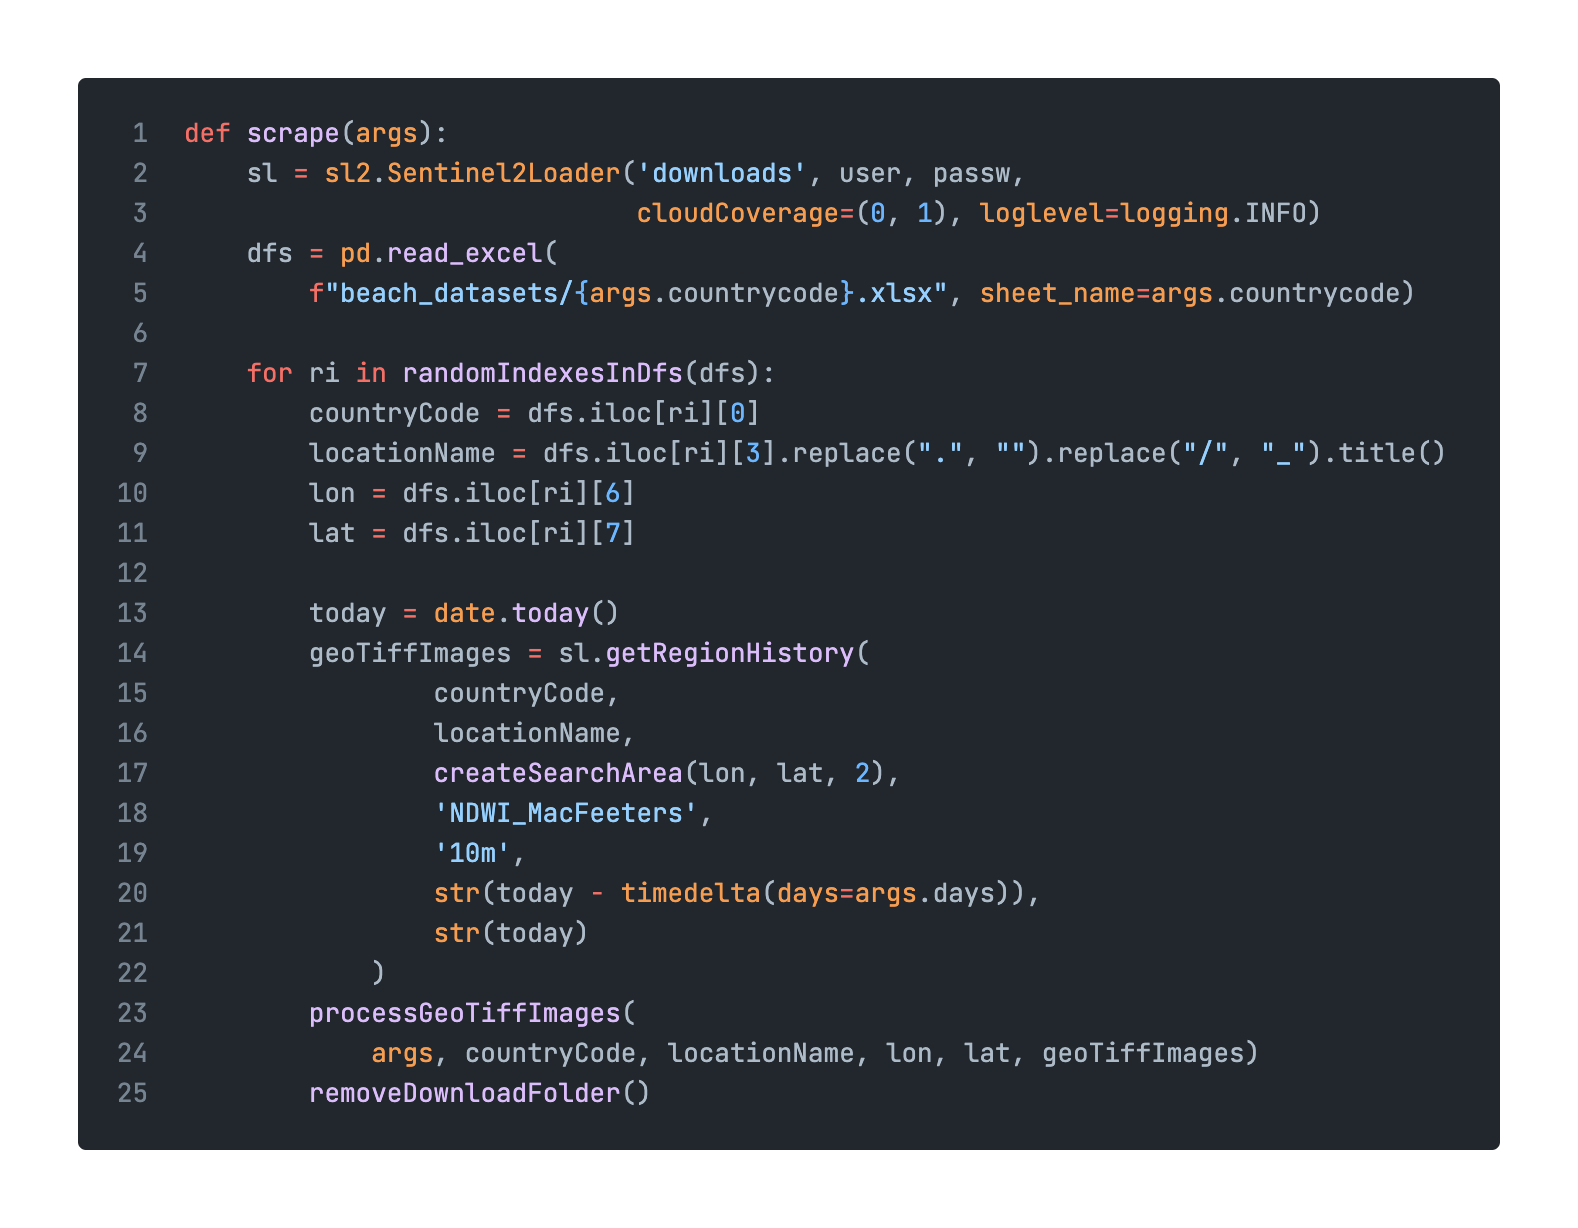
\includegraphics[width=\textwidth]{sentinel-satellite-scraper-scrape.png}
    \caption{The \emph{scrape(args)} methodh that is the entry point of the \acrshort{sss}.}
    \label{fig:sentinel-satellite-scraper-scrape}
\end{figure}

The scraping method first instantiates the \emph{Sentinel2Loader} from the \emph{sentinelloader} library with the folder to download products too, the Copernicus user, the desired cloud coverage percentage, and the log level. After initialisation the locations to scrape for are read in from one of many excel files located in the scrapers directory. Each of these Excel files contains geo-locations on beaches in a specific country and come from a publicly available dataset from the European Environmental Agency \cite{bathing_dateset}. 

When the Excel data has been read to memory, the main scraping loop begins, where it randomly selects a non-processed beach and proceeds. Randomly selecting a beach is a deliberate choice as the Copernicus API restricts the number of offline products that can be downloaded to 20 each day. Mixing up which locations we query historical data from ensures we use the offline product retrievals differently each time the script is run. Thus, we improve the chances of getting historical data for different areas over time.

Next, the different needed parameters are extracted from the excel data, and the process of downloading products, combining bands, and cropping the resulting images is started by the \emph{getRegionHistory(...)} method call. This call is called with the country code, the location name, a search area that defines the boundary of the location of interest, the index we want to combine bands, the spatial resolution, the from date, and lastly, the to date.

As indicated by the ``NDWI\_MacFeeters`` parameter, the combination of bands happens accordingly to the \acrfull{ndwi} \cite{ndwi}. The MacFeeters formula for \acrshort{ndwi} combines the bands into an image that differentiates water from land. The \acrshort{ndwi} uses a simple formula to combine band 3 and band 8 to give a value between 0 and 1 for each pixel that indicates how likely that pixel is to be either water or land. \cite{sentinel-2-bands-combinations}

\[ NDWI = \dfrac{B3 - B8}{B3 + B8} \]

Furthermore, the cropping of the image relies on the provided search area that defines the boundaries of the location of interest. \emph{Sentinelloader} automatically crops out the area of interest from the downloaded product(s). In cases where the place of interest covers multiple products, the \emph{sentinelloader} library can download, combine and crop the image from various products, so no data is lost.

After having downloaded products, combined bands, and cropped the resulting image, custom pre-processing is done on the resulting image to color it based on the \acrshort{ndwi} values and to ensure the image size is as compact as possible. This work happens in the \emph{processGeoTiffImages(...)}.

\begin{figure}[h!]
    \centering
    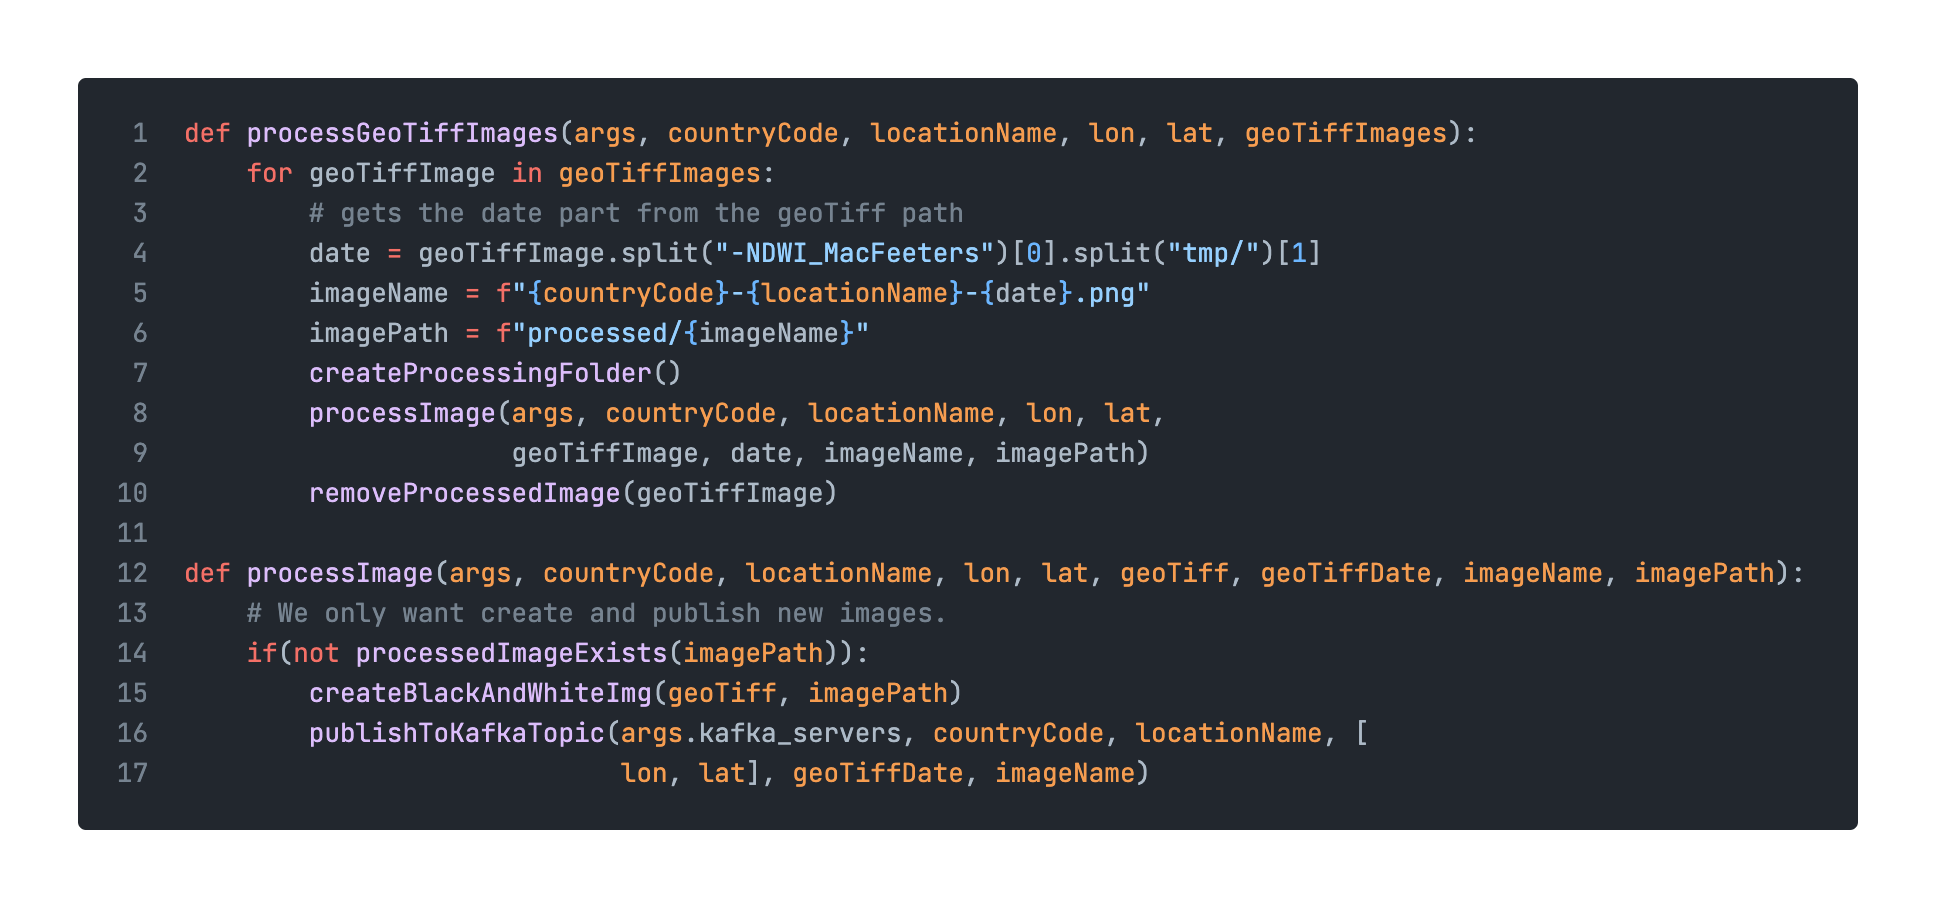
\includegraphics[width=\textwidth]{sentinel-satellite-scraper-pre-processing.png}
    \caption{The \emph{scrape(args)} method that is the entry point of the \acrshort{sss}.}
    \label{fig:sentinel-satellite-scraper-pre-processing}
\end{figure}

First, the desired image name and path of the pre-processed images are constructed from the downloaded images from the \emph{sentinelloader}. Then the downloaded images are passed on to the \emph{processImage(...)} method that first creates a new image from one of the downloaded images. The new image is combined with a black and white color map that paints any pixel with an \acrshort{ndwi} value greater than 0.6 white, and any pixel with an \acrshort{ndwi} value smaller than 0.6 black. Two of these images can be seen in \autoref{fig:sentinel-satellite-scraper-processed-image}.

\begin{figure}[h!]
    \centering
    \fbox{
\includegraphics[width=0.4\textwidth]{DK-EJERSLEVLYNG-2021-10-13.png}}
    \fbox{
\includegraphics[width=0.4\textwidth]{DK-GLSTRANDSKOV-2021-09-08.png}}
    \caption{Processed images of Ejerslevlyng (left) and Gl Strandskov (right) beaches in DK with the black and white colormap applied.}
    \label{fig:sentinel-satellite-scraper-processed-image}
\end{figure}

Finally, the image and relevant metadata are compressed to JSON and published to Kafka. After this, all downloaded satellite imagery is deleted to clear up valuable space for processing the following location. If this cleanup process is skipped, the downloaded products would quickly fill up the remaining disk space on the machines where the script is run.

\subsection{Spark NDWI Analyzer}\label{subsec:ndwi-analyzer}

The Spark NDWI Analyzer is a python spark job created to continuously consume and analyze messages from Kafka to provide insight into what the scraped satellite images can tell us about the water content changes. EcoBeach relies on distributed Spark workers to handle this job, to efficiently analyze newly scraped satellite images, and feed the results back to Kafka.\\\\
\noindent
The Spark NDWI Analyzer runs constantly and watches for changes to the Kafka topic ``ndwi\_images``. Whenever a new message is added to the topic, the Spark NDWI Analyzer consumes this message, analyzes it, and produces a new message to the ``ndwi\_results`` topic that holds all data that the data pipeline has fully processed.\\\\
\noindent
The analysis is a three-step process. First the black and white images in \autoref{fig:sentinel-satellite-scraper-processed-image} that are created by the \acrshort{sss} are recreated. The images are stored in the Kafka message that contains the image encrypted as byte64. Then all white and black pixels are counted in the image, and lastly, the percentage and area (in cubic meters) of both white (water) and black (land) pixels are calculated. The relevant code is shown in \autoref{fig:ndwi-analyzer-code}.

\begin{figure}[H]
    \centering
    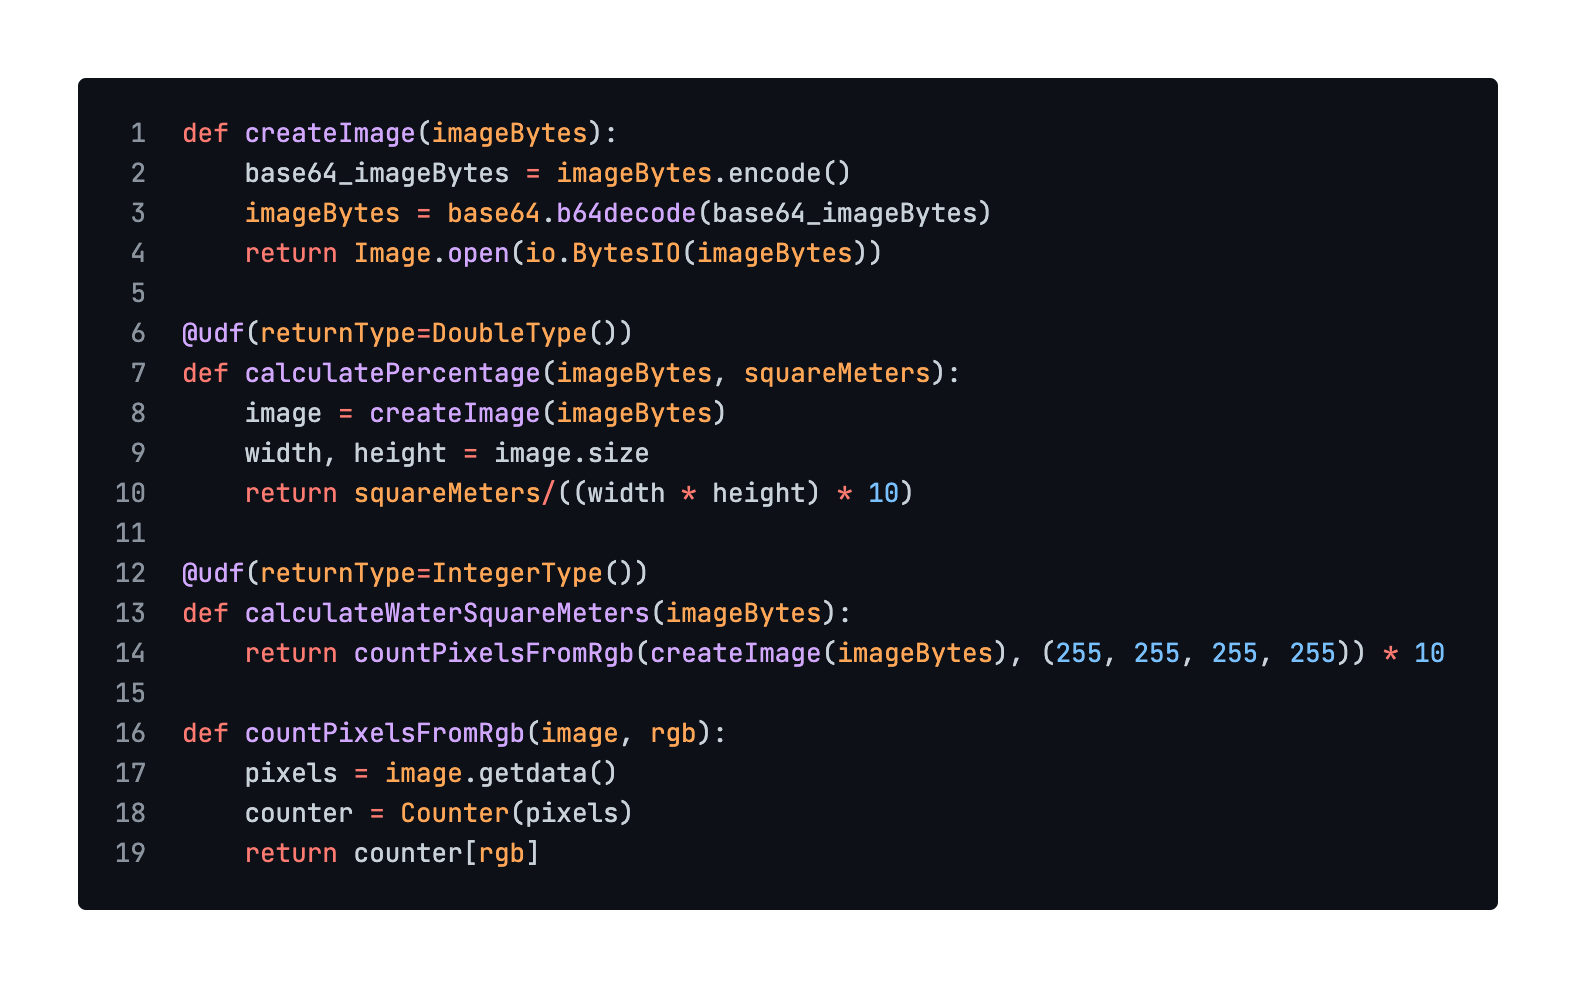
\includegraphics[width=\textwidth]{ndwi-analyzer-code.png}
    \caption{The code that recreates the black-and-white images, counts pixels and calculates percentage and area (in cubic meters) of water and land.}
    \label{fig:ndwi-analyzer-code}
\end{figure}

\subsection{WebAPI}

Our system requires a Web API to handle the data flow between the Android application and the database. This is first and foremost done to increase security and prevent any direct access to the database from the application. In our case, our application only requests data from the API, it does not add or change any items in the database, so this is a one-way dataflow.

The API accesses the MongoDB database via MongoDB Driver which is an Object–relational mapping (ORM) tool that we use to map data coming from the database to actual Beach objects which the API can handle, process and send as Json objects to endpoint-callers. 

The API is deployed in a Docker container for easier testing and configurability. The database connection string can then be set in a system environment variable when launching the container. Once the container is running data can be requested on two endpoints.

\subsubsection{/api/Beach}

The application can call the API to request all the stored beach data from the database. This is first used when the application has to display the pins on the map, indicating the locations of all the beaches. The requested data is sent by the API in a JSON format, which is processed by the Android application into actual Beach objects.

\subsubsection{/api/Beach/{id}}

The application can also call an API request to get a single beach item from the database, based on the provided ID. This call is used when the user selects a beach in the application, and the detailed information is requested to display it for the user. 

\subsubsection{Architecture}

The backend services hosting the API is a multi-tier architecture system which breaks down into three main components:

\begin{itemize}
    \item Presentation Tier – in this system’s case, it contains the hosted API which can be called externally. It contains the controllers that handle all the API requests received.
    \item Logic Tier – This tier mainly contains the models and helper classes. Models describe the type of object the ORM should map the data from the database. Also provides methods to read files with .csv extensions and use them to seed an empty database with beaches from the environmental agency’s dataset.
    \item Data Tier – Provides services and context for the backend to reach the MongoDB database and queries it for data when needed. 
\end{itemize}

Introducing multiple tiers in our architecture allows us to have a very decoupled system in case a tier needs to be changed, or used in another system of similar kind. 

\begin{figure}[H]
    \centering
    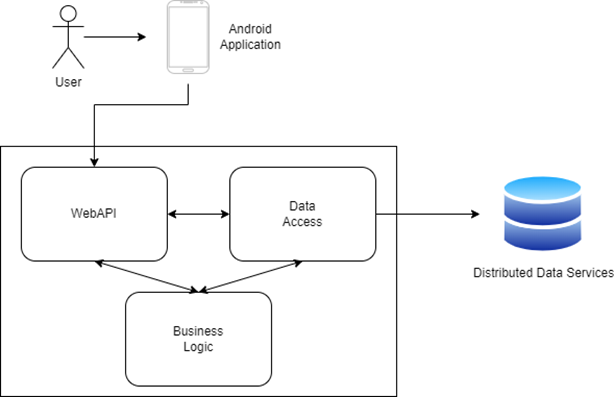
\includegraphics[width=12cm]{api_architecture.png}
    \caption{WebAPI Multi-layer architecture}
    \label{fig:api_architecture}
\end{figure}

\subsection{EcoBeach App}\label{subsec:ecobeach-app}

\subsubsection{Activities and layouts}

The most important component of an application is the Activity, which is not only responsible for the user interface, but also for the operation of the application itself. During the implementation, three Activities have been created. These activities are the followings:

\begin{itemize}
    \item SplashScreenActivity - After starting the application this is the first thing that the user can see for two seconds. On the centre of the screen there is the logo of the application and below that, there is the name of the application. We used Constraint layout, which is one of the latest and most efficient layout types.
    \item MainActivity - In this activity the user can see the Google Maps, with markers, that shows the different beaches in Europe. At first, it is going to focus on the user’s location.
    \item BeachActvity - Here you can see more information about a specific beach and can see a satellite map focused on the location.
\end{itemize}

Each activity has their own layout, on the following pictures, you can see three screenshots of the different layouts.


\begin{figure}[h!]
    \centering
    \fbox{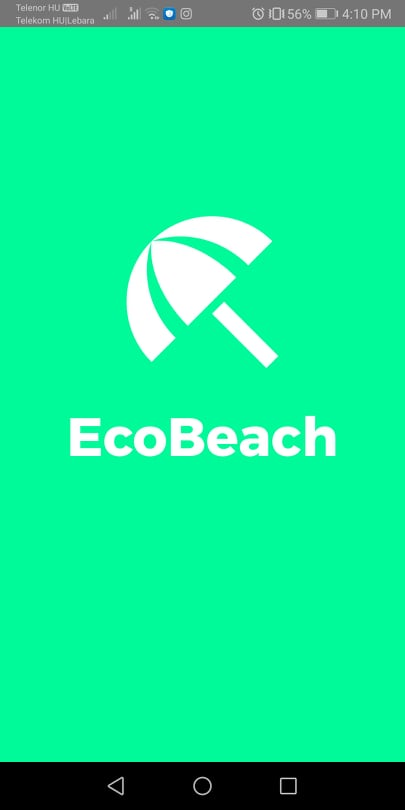
\includegraphics[width=0.3\textwidth]{splash_activity.jpg}}
    \fbox{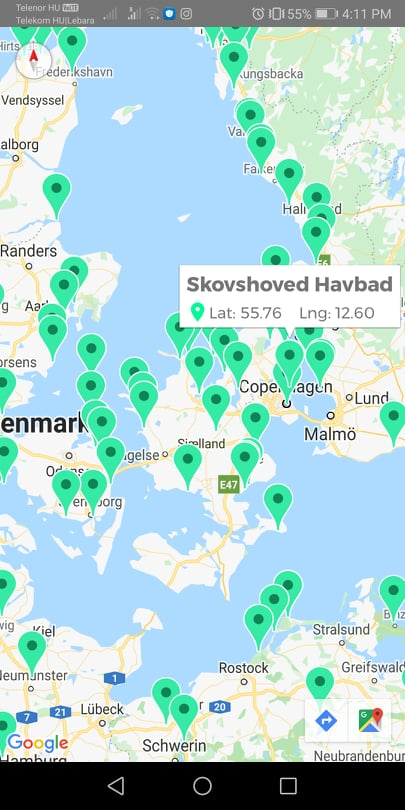
\includegraphics[width=0.3\textwidth]{main_activity.jpg}}
    \fbox{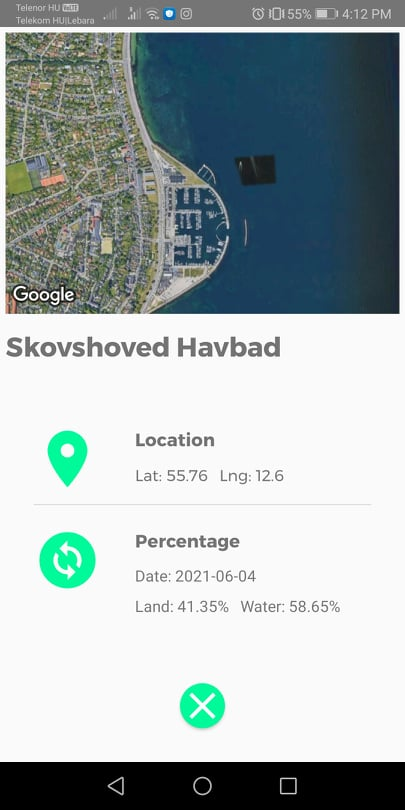
\includegraphics[width=0.3\textwidth]{beach_activity.jpg}}
    \caption{Screenshots of SplashScreenActivity (left), MainActivity (center) and BeachActivity (right).}
    \label{fig:activities}
\end{figure}

\subsubsection{Navigation}

On \autoref{fig:navigation}, the navigation between the activities is shown. After starting the application, the users can see the SplashScreen Activity for two seconds, then they are navigated to the MainActivity, which shows them the marked Google Maps. Clicking on a marked place the user is navigated to the BeachActivity, where they can be informed about the beach, like the name of the beach, the coordinates, and about the shoreline changes.

Having Internet and location enabled are very important, so in the MainActivity both are checked. If either the Internet or the location is not enabled, the user receives an alert, and the application is closed.

\begin{figure}[H]
    \centering
    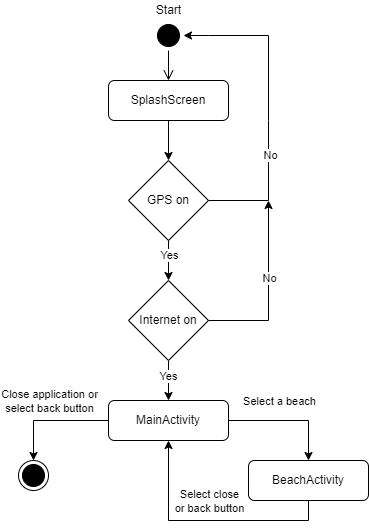
\includegraphics[width=8.5cm]{navigation.png}
    \caption{Navigation between the Activities.}
    \label{fig:navigation}
\end{figure}

\subsubsection{User permissions}

Three permissions are needed to use this application. These permissions can be seen on \autoref{fig:user_permissions}.

\begin{figure}[h!]
    \centering
    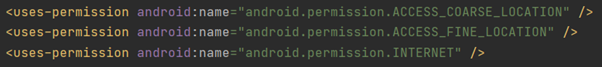
\includegraphics[width=\textwidth]{user_permissions.png}
    \caption{The user must grant these permissions in order to use the EcoBeach application.}
    \label{fig:user_permissions}
\end{figure}

Location permissions are needed for getting the user’s location. If the user is not accepting it, then the application is closed automatically, since the app is based on having the location permission.

Internet is needed for Google Maps, so that we can display different beaches on the map. Without this, we are unable to show the map in the MainActivity. However, the internet is not only used for Google Maps, but also for the Web API.

